\input ../SlidePreamble
\input ../preamble


\begin{document}

{\Huge

  \centerline{\bf TTIC 31230, Fundamentals of Deep Learning}
  \bigskip
  \centerline{David McAllester, Winter 2018}
  \vfill
  \centerline{Entropy and Compressibility}
  \vfill
  \centerline{Rate-Distortion Autoencoders}

\slide{Big Picture: Cross-Entropy as a Data Rate}

For a distribution $P(y)$ on a discrete set ${\cal Y}$, the entropy $H(P)$, when measured using $\log_2$ rather than $\ln$, gives the number of bits needed
on average, when drawing from $P$, to represent the elements of ${\cal Y}$.

\vfill
The cross-entropy $H(P,Q)$ give the number of bits used to code for items drawn from $P$ but using the code defined by $Q$.

\vfill
Cross-entropy gives the ``data rate'' when transmitting codes for items drawn from $P$ but using the code defined by $Q$.

\slide{Entropy and Compressibility}

Let $S$ be a finite set.

\vfill
Let $z$ be a compression (or coding) function  assigning a bit string $z(y)$ to each $y \in S$.

\vfill
The compression function $z$ is called {\em prefix-free} if for $y' \not = y$ we have that $z(y')$ is not a prefix of $z(y)$.

\slide{Prefix-Free Codes as Probabilities}

A prefix-free code defines a binary branching tree --- branch on the first code bit, then the second, and so on.

\vfill
For a prefix-free code, only the leaves of this tree can be labeled with the elements of $S$.

\vfill
The code defines a probability distribution on $S$ by randomly selecting branches.

\vfill
We have $P_z(y) = 2^{-|z(y)|}$.

\slide{Bits vs. Nats}

We have that $|z(y)|$ is a number of bits.

\vfill
We can define entropy in units of bits by

\vfill
$$H_2(y) = E_y\; - \log_2 P(y) = H(y)/(\ln \;2)$$

\vfill
If $y$ is uniformly distributed over 8 values then $H_2(y)$ is 3 bits.

\vfill
We have that $H_2(y)$ is a number of bits while $H(y)$ is a number of ``nats''.

\slide{The Source Coding (compression) Theorem}

(1) There exists a prefix-free code $z$ such that
$$|z(y)| <= (- \log_2 \mathrm{Pop}(y)) + 1$$
and hence
$$E_{y\sim \mathrm{Pop}} |z(y)| \leq H_2(\mathrm{Pop}) +1$$

\vfill
(2) For any prefix-free code $z$

$$E_{y \sim \mathrm{Pop}}\;|z(y)| \geq H_2(\mathrm{Pop})$$

\slide{Code Construction}

\vfill
We construct a code by iterating over $y \in S$ in order of decreasing probability (most likely first).

\vfill
For each $y$ select a code word $z(y)$ (a tree leaf) with length (depth)

\vfill
$$|z(y)| = \lceil - \log_2 \mathrm{Pop}(y)\rceil$$

\vfill
and where $z(y)$ is not an extension of (under) any previously selected code word.

\slide{Code Existence Proof}

At any point before coding all elements of $S$ we have
$$\sum_{y \in \mathrm{Defined}} 2^{-|z(y)|} \leq \sum_{y \in \mathrm{Defined}} \mathrm{Pop}(y) < 1$$

\vfill
Therefore there exists an infinite descent into the tree that misses all previous code words.

\vfill
Hence there exists a code word $z(x)$ not under any previous code word with
$|z(x)| = \lceil - \log_2 \mathrm{Pop}(y)\rceil$.

\vfill
Furthermore $z(x)$ is at least as long as all previous code words and hence $z(x)$ is not a prefix of any previously selected code word.

\slide{No Better Code Exists}

Let $z$ be an arbirtary coding.

\begin{eqnarray*}
E_y\;|z(y)| & = & E_y\; -\log_2 P_z(y) \\
\\
 & = & H_2(\mathrm{Pop},P_z) \\
 \\
 &= & H_2(\mathrm{Pop}) + KL_2(\mathrm{Pop},P_Z) \\
 \\
 &\geq & H_2(\mathrm{Pop})
\end{eqnarray*}
 
\ignore{
\slide{Huffman Coding}

Maintain a list of trees $T_1,\;\dots,\;T_N$.

\vfill
Inititally each tree is just one root node labeled with an element of $S$.

\vfill
Each tree $T_i$ has a weight equal to the sum of the probabilities of the nodes on the leaves of that tree.

\vfill
Repeatedly merge the two trees of lowest weight into a single tree until all trees are merged.

\slide{Optimality of Huffman Coding}

{\bf Theorem}: The Huffman code $T$ for $\mathrm{Pop}$ is optimal --- for any other tree $T'$ we have $d(T;\mathrm{Pop}) \leq d(T';\mathrm{Pop})$.

\vfill
{\bf Proof}: The algorithm maintains the invariant that there exists an optimal tree including
all the subtrees on the list.

\vfill
To prove that a merge operation maintains this invariant we consider any tree containing the given subtrees.

\vfill
Consider the two subtrees $T_i$ and $T_j$ of minimal weight.  Without loss of generality we can assume that $T_i$ is at least as deep as $T_j$.

\vfill
Swapping the sibling of $T_i$ for $T_j$ brings $T_i$ and $T_j$ together and can only improve the average depth.

\slide{Optimality of Huffman Coding}

Why the swap operation cannot increase entropy. ...
}

\slide{Big Picture: Differential Entropy is Always Infinite}

For a continuous set ${\cal Y}$ (such as the unit interval on real numbers)
and for any probability density (smooth measure) on ${\cal Y}$ the probability of
any single point $y \in {\cal Y}$ is zero.

\vfill
This implies that the entropy is infinite --- it takes an infinite number of bits to represent
a random real number.

\vfill
Cross-entropy between continuous densities is also always infinite and {\color{red} differential cross-entropy loss is not meaningful.}

\slide{Differential Entropy}

Consider a continuous density $p(x)$.  For example

\vfill
$$p(x) = \frac{1}{\sqrt{2\pi}\; \sigma}\; e^{\frac{-x^2}{2\sigma^2}}$$

\vfill
Differential entropy is often defined as

\vfill
$$H(p) \doteq \int \left(\ln \frac{1}{p(x)}\right) p(x) dx$$

\slide{Finite Differential Entropy is Not Meaningful}

\begin{eqnarray*}
  H({\cal N}(0,\sigma)) & = &  + \int \left( \ln(\sqrt{2\pi} \sigma) + \frac{x^2}{2\sigma^2}\right) p(x) dx \\
  \\
  & = & \ln(\sigma) + \ln(\sqrt{2\pi}) + \frac{1}{2}
\end{eqnarray*}

\vfill
But if we take $y \doteq x/2$ we get $H(y) = H(x) - \ln 2$.

\vfill
Also for $\sigma << 1$, we get $H(p) < 0$

\vfill
Hence differential entropy then depends on the choice of units --- a distributions on lengths will have a different entropy
when measuring in inches than when measuring in feet.

\slide{Differential Entropy is Always Infinite}

Consider quantizing the the real numbers into bins.

\vfill
A continuous probability densisty $p$ assigns a probability $p(B)$ to each bin.

\vfill
As the bin size decreases toward zero the entropy of the bin distribution increases toward $\infty$.

\vfill
A meaningful convention is that $H(p) = +\infty$ for any continuous density $p$.

\slide{Differential KL-divergence is Meaningful}

$$KL(p,q) = \int \left( \ln \frac{p(x)}{q(x)}\right) p(x) dx$$

\vfill
This integral can be computed by dividing the real numbers into bins and computing the $KL$ divergence between the distributions on bins.

\vfill
The KL divergence between the bin distribution typically approaches a finite limit as the bin size goes to zero.

\slide{KL-Divergence can also be Infinite}

$$KL(p,q) = E_{x \sim p}\; \log\frac{p(x)}{q(x)}$$
\vfill
In either the discrete or continuous case, if a set is assigned nonzero probability by $p$ but zero probability by $q$ then $KL(p,q) = +\infty$.

\vfill
If every set assigned nonzero probability by $p$ is also assigned nonzero probability by $q$ then we say that $p$ is absolutely continuous with respect to $q$.

%the slides on rate-distortion example need more detail.  Every slide should be at least doubled.
% it also needs more material.  A theorem on noise in latent variables would be nice.

\slide{Big Picture: Unsupervised Learning}

\centerline{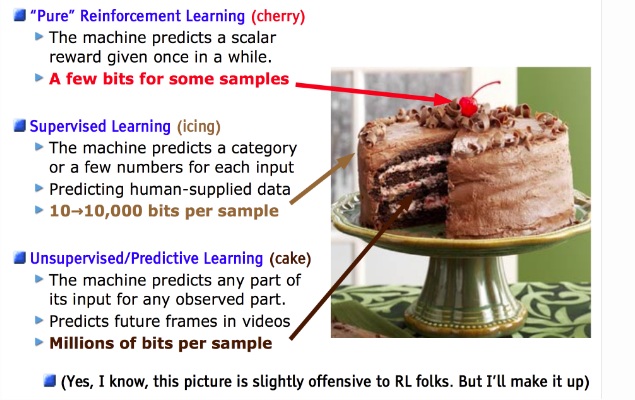
\includegraphics[width = 6in]{../images/cake}}

\vfill
Consider the power of BERT.

\vfill
We would like to density estimation for images and sound waves.

\slide{The Big Picture: Rate-Distortion Loss}
For density estimation of naturally occurring continuous distributions we consider
a parameterized ``rounding'' operation mapping $y$ to $\tilde{y}_\Phi(y)$ with $\tilde{y} \in {\cal Y}$ for ${\cal Y}$ discrete.

\vfill
We then define rate-distortion loss

\vfill
$${\cal L}(\Phi) = E_{y \sim \mathrm{Pop}}\;(- \ln P_\Phi(\tilde{y}_\Phi(y))) + \lambda D(y,\tilde{y}_\Phi(y))$$

\vfill
where $D(y,\tilde{y})$ is some ``distortion function'' measuring a distance between $y$ and $\tilde{y}$.

\slide{The Rate-Distortion Tradeoff}

$${\cal L}(\Phi) = E_{y \sim \mathrm{Pop}}\;(- \ln P_\Phi(\tilde{y}_\Phi(y))) + \lambda D(y,\tilde{y}_\Phi(y))$$

\vfill
The first term is just cross-entropy loss which we are calling the ``rate''.  This terminology is explained below.

\vfill
The meta-parameter $\lambda$ controls the trade off between rate and distortion.


\slide{Common Distortion Functions}

$$\Phi^* = E_{y \sim \mathrm{Pop}}\;(- \ln P_\Phi(\tilde{y}_\Phi(y))) + \lambda D(y,\tilde{y}_\Phi(y))$$

\vfill
It is common to take

$$D(y,\tilde{y}) = ||y-\tilde{y}||^2 \hspace{4em}(L_2)$$

\vfill
or

$$D(y,\tilde{y}) = ||y-\tilde{y}||_1 \hspace{4em} (L_1)$$

\slide{Rate-Distortion Autoencoders}

Given a continuous signal $y$ we can compress it into a (discrete) bit string $\tilde{z}_\Phi(y)$.

\vfill
We let $\tilde{y}_\Phi(\tilde{z}_\Phi(y))$ be the decompression of $\tilde{z}_\Phi(y)$.

\vfill
Rate-Disrtion loss can then be written as

$${\cal L}(\Phi) = E_{y \sim \mathrm{Pop}}\;|\tilde{z}_\Phi(y)| + \lambda D(y,\tilde{y}(\tilde{z}(y)))$$

\slide{A Case Study in Image Compression}

{\bf End-to-End Optimized Image Compression, Balle, Laparra, Simoncelli, ICLR 2017.}


\vfill
$${\color{red}y \hspace{5em}  \tilde{z}_\Psi(y) \hspace{4em} \tilde{z} \hspace{6em} \tilde{y}_\Phi(\tilde{z}) \hspace{4em}||y - \tilde{y}||^2}$$
\centerline{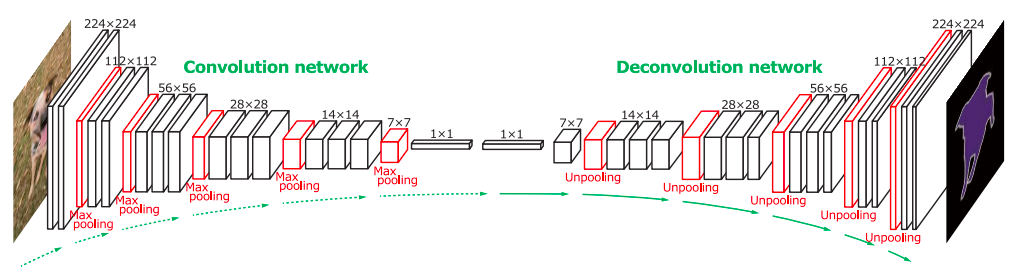
\includegraphics[width=9in]{../images/Deconv}}

\vfill
The model described here has been simplified from the original.


\anaslide{JPEG at 4283 bytes or .121 bits per pixel}

\bigskip
\centerline{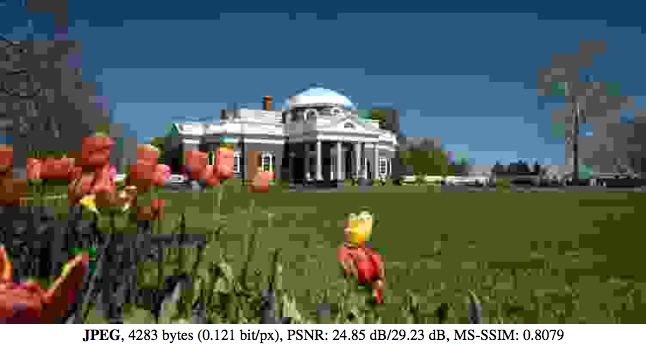
\includegraphics[height=5in]{../images/RateDist2}}

\anaslide{JPEG 2000 at 4004 bytes or .113 bits per pixel}

\bigskip
\centerline{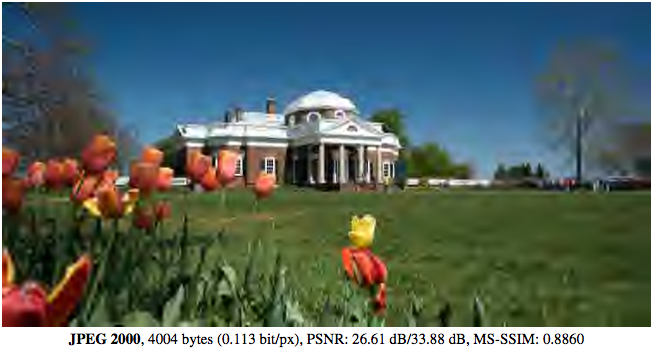
\includegraphics[height= 5in]{../images/RateDist3}}

\anaslide{Deep Autoencoder at 3986 bytes or .113 bits per pixel}

\bigskip
\centerline{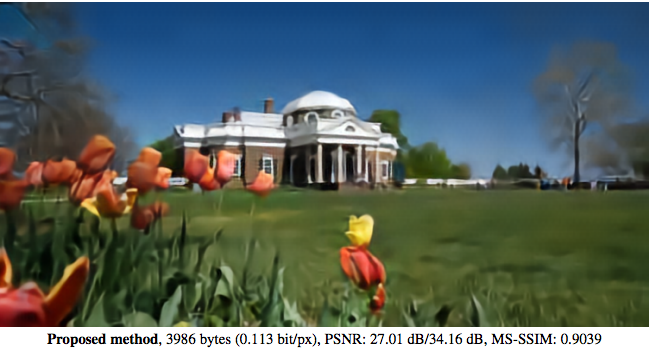
\includegraphics[height = 5in]{../images/RateDist4}}

\slide{The Encoder $z_\Phi(y)$}

This paper uses a three layer CNN for the encoder.

\vfill
The first layer is computed stride 4.

\vfill
The two remaining layers are computed stride 2.

\slide{The number of numbers}

\vfill
The first layer is computed stride 4.

\vfill
The next two layers are computed stride 2.

\vfill
Final image dimension is reduced by a factor of 16 with 192 channels per pixel (192 channels is for color images).

\vfill
$$192 < 16 \times 16 \times 3 = 768$$

\vfill
The final values $z[x,y,i]$ are rounded to integers $\tilde{z}[x,y,i]$.

\slide{Increasing Spatial Dimension in Decoding}

\centerline{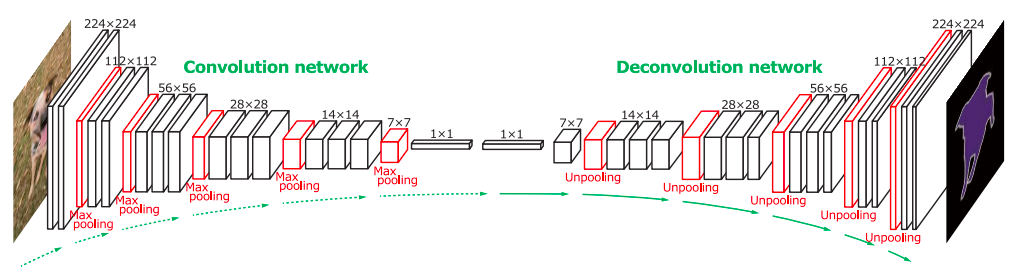
\includegraphics[width=9in]{../images/Deconv}}
\centerline{[Hyeonwoo Noh et al.]}

\vfill
In the ICLR 17 paper the deconvolution network has the shape as the input CNN but with independent parameters.

\slide{Increasing Spatial Dimensions in Deconvolution}

Consider a stride 2 convolution
\begin{eqnarray*}
  L_{\ell+1}[x,y,j] & = & \sigma\left(\sum_{\Delta x,\Delta y,i}   W[\Delta x, \Delta y, i,j] L_\ell[2x + \Delta x, 2y + \Delta y, i]\right)
\end{eqnarray*}

\vfill
For deconvolution we use stride 1 with 4 times the features.
\begin{eqnarray*}
  L'_\ell[x,y,i] & = & \sigma\left(\sum_{\Delta x,\Delta y,j}   W[\Delta x, \Delta y, j,i] L'_{\ell+1}[x + \Delta x, y + \Delta y, j]\right)
\end{eqnarray*}

\vfill
The channels at each $L'_\ell[x,y]$ are divided among four higher resolution pixels.

\vfill
This is done by a simple reshaping of $L'_\ell[x,y,i]$.

\slide{Rate-Distortion Autoencoders}

$$\Phi^* = \argmin_\Phi \;E_{y \sim \pop}\;|\tilde{z}_\Phi(y)| + \lambda D(y,\tilde{y}_\Phi(z_\Phi(y)))$$

\vfill
Oops: Because of rounding, $\tilde{z}_\Phi(y)$ is discrete and the gradients are zero.

\vfill
Note, however that the rate-distortion loss is measurable.

\vfill
We will approximate the gradient descent but still be able to measure loss.

\slide{Rate-Distortion Autoencoders}

\begin{eqnarray*}
\Phi^* & & = \argmin_\Phi {\cal L}_{\mathrm{rate}}(\Phi) + \lambda {\cal L}_{\mathrm{dist}} (\Phi) \\
\\
{\cal L}_{\mathrm{rate}}(\Phi) & = & E_{y \sim \pop}\;|\tilde{z}_\Phi(y)| \\
\\
{\cal L}_{\mathrm{dist}}(\Phi) & = & E_{y \sim \mathrm{Pop}} \;D(y,\tilde{y}_\Phi(\tilde{z}_\Phi(y)))
\end{eqnarray*}

\vfill
We will consider differentiable approximations to both ${\cal L}_{\mathrm{rate}}$ and ${\cal L}_{\mathrm{dist}}$.

\slide{A Differentiable Approximation of ${\cal L}_{\mathrm{rate}}$}

\begin{eqnarray*}
{\cal L}_{\mathrm{rate}}(\Phi) & = & E_{y \sim \pop}\;|\tilde{z}_\Phi(y)| 
\end{eqnarray*}

\vfill
Recall that $\tilde{z}(y)$ is a rounding of a continuous tensor $z[x,y,i]$.

\vfill
We can use the differentiable approximation

\vfill
$$|\tilde{z}_\Phi(y)| \approx \sum_{x,y,i} \; \max(0,\log_2 z_\Phi[x,y,i])$$

\vfill
This can be viewed as approximating a discrete entropy with differential entropy.

\slide{Differential Entropy vs. Discrete Entropy}

\bigskip
\centerline{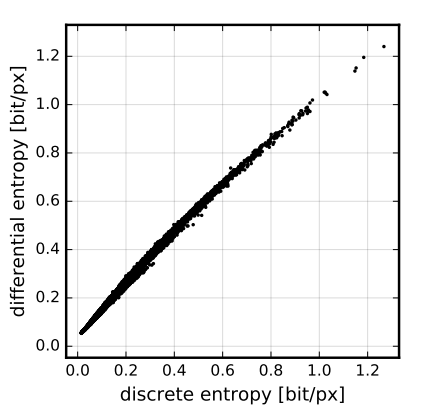
\includegraphics[height=5in]{../images/RateDist6}}

\slide{A Differentiable Approximation of ${\cal L}_{\mathrm{dist}}$}

\begin{eqnarray*}
{\cal L}_{\mathrm{dist}}(\Phi) & = & E_{y \sim \mathrm{Pop}} \;D(y,\tilde{y}_\Phi(\tilde{z}_\Phi(y))) \\
\\
& \approx & E_{y,\epsilon} \;D(y,\;\tilde{y}(z_\Phi(y) + \epsilon))
\end{eqnarray*}

\vfill
Here $\epsilon$ is a noise tensor with $\epsilon[x,y,i]$ drawn uniformly form $(-1/2,1/2)$.

\slide{Noise vs. Rounding}

\centerline{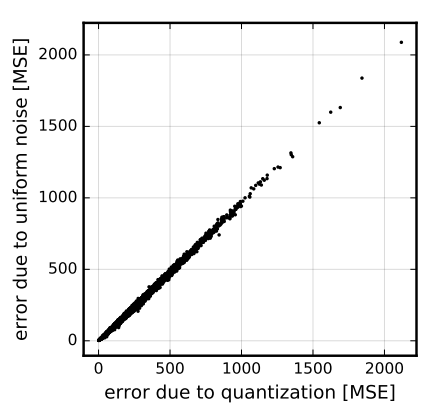
\includegraphics[height=5in]{../images/RateDist5}}


\slide{Varying the Level Of Compression}

$$\Phi^* = \argmin_\Phi\; E_{y \sim \mathrm{Pop}} |\tilde{z}_\Phi(y)| + \frac{1}{2}{\color{red} \lambda} ||y - \tilde{y}_\Phi(\tilde{z}_\Phi(y))||^2$$

\vfill
Different levels of compression correspond to different values of $\lambda$.

\vfill
In all levels of compression we replace 768 numbers by 192 numbers.

\vfill
Higher levels of compression result in smaller integer values in the 192 numbers.

\slide{Conditional Rate-Distortion Autoencoders}

$$\Phi^* = \argmin_\Phi \;\;E_{(x,y) \sim \pop} \;\;\; |\tilde{z}_\Phi(y|x)|\; + \; \lambda D(y\;|\;\tilde{y}_\Phi(x,\tilde{z}_\Phi(y|x)))$$

\slide{Colorization}

\centerline{\includegraphics[height = 2in]{../images/colorization}}

\vfill
$${\color{red} \Phi^* = \argmin_\Phi E_{(x,y) \sim \mathrm{Pop}}\;|\tilde{z}_\Phi(y|x)| + \frac{1}{2}\lambda ||y - \tilde{y}_\Phi(x,\tilde{z}_\Phi(y|x))||^2}$$

\vfill
If the image can be segmented based on $x$ then $\tilde{z}_\Phi(y|x)$ can be a specification of color of each segment --- this would be very compact.


\slide{END}

}
\end{document}

